\documentclass[11pt]{beamer}
\usetheme{Luebeck}
%\usecolortheme{seahorse}
\useinnertheme{rectangles}
\useoutertheme{infolines}
\usepackage{xcolor, natbib}
\usepackage[utf8]{inputenc}
\usepackage{tikz}
\usepackage{tabularx}
\usepackage{lipsum}
\usepackage{amsmath,graphicx,dsfont}
\usepackage{graphicx}
\usetikzlibrary{shapes,backgrounds,arrows,automata,snakes,shadows,positioning, mindmap}
%===================================
\newcommand\betab{{\boldsymbol{\beta}}}
\newcommand\thetab{{\boldsymbol{\theta}}}
\newcommand\Sigmab{{\boldsymbol{\Sigma}}}
\newcommand\Yb{{\bf Y}}
\newcommand\Zb{{\bf Z}}
%===================================
\newcommand{\Ccal}{\mathcal{C}}
\newcommand{\edgeunit}{1.5}
\newcommand{\emphase}[1]{\textcolor{Complement}{#1}}
\newcommand{\bleu}[1]{\textcolor{Framableulight}{#1}}
\newcommand{\pos}[1]{\textcolor{Darkgreen}{#1}}
\newcommand{\nega}[1]{\textcolor{Nicered}{#1}}
\newcommand{\independent}{\perp \!\!\! \perp}

\newcommand{\Ncal}{\mathcal{N}}
\tikzset{%
    observed/.style={%
    scale=0.6,circle,draw=Framableulight,transform shape,fill=white,font=\Large}
}
\tikzset{%
    basic/.style={%
    scale=0.4,circle,draw=Framableu,transform shape,fill=Framableulight,font=\small}
}
\newcommand{\argmax}{\mathop{\mathrm{argmax}}}   
\newcommand{\backupbegin}{
   \newcounter{framenumberappendix}
   \setcounter{framenumberappendix}{\value{framenumber}}
}
\newcommand{\backupend}{
   \addtocounter{framenumberappendix}{-\value{framenumber}}
   \addtocounter{framenumber}{\value{framenumberappendix}} 
}

\makeatletter
\setbeamertemplate{footline}
{
  \leavevmode%
  \hbox{%
  \begin{beamercolorbox}[wd=.333333\paperwidth,ht=2.25ex,dp=1ex,center]{author in head/foot}%
    \usebeamerfont{author in head/foot}Mixture of trees for network inference%~~\beamer@ifempty{\insertshortinstitute}{}{(\insertshortinstitute)}
  \end{beamercolorbox}%
  \begin{beamercolorbox}[wd=.333333\paperwidth,ht=2.25ex,dp=1ex,center]{title in head/foot}%
    \usebeamerfont{title in head/foot} Networking days
  \end{beamercolorbox}%
  \begin{beamercolorbox}[wd=.333333\paperwidth,ht=2.25ex,dp=1ex,right]{date in head/foot}%
    \usebeamerfont{date in head/foot}\insertshortdate{}\hspace*{2em}
    \insertframenumber{} / \inserttotalframenumber\hspace*{2ex} 
  \end{beamercolorbox}}%
  \vskip0pt%
}
\makeatother
%===================================
\definecolor{Framableu}{RGB}{12,91,122}
\definecolor{Framableulight}{RGB}{18,144,176}
\definecolor{Nicered}{RGB}{176,18,65}
%\definecolor{Nicered}{RGB}{141,14,52}
\definecolor{Lightpink}{RGB}{229,177,218}
\definecolor{Green}{RGB}{144,176,18}
\definecolor{Lightcomplement}{RGB}{235,204,196}
\definecolor{Darkgoldenrod}{RGB}{176,144,18}
\definecolor{Darkomplement}{RGB}{122,43,12}
\definecolor{Complement}{RGB}{176,50,18}
\definecolor{Darkgreen}{RGB}{52,141,14}
%===================================
\setbeamertemplate{itemize items}[square]
\setbeamertemplate{blocks}[shadow=false]
\setbeamertemplate{caption}{\raggedright\insertcaption\par}
%===================================
\setbeamercolor{section in head/foot}{fg=white,bg=Framableu}
\setbeamercolor{subsection in head/foot}{fg=white,bg=Framableulight}
\setbeamercolor{author in head/foot}{bg=Framableu}
\setbeamercolor{item}{fg=Framableulight}
\setbeamercolor*{structure}{bg=Framableulight!20,fg=Framableulight}
\setbeamercolor*{palette secondary}{use=structure,fg=white,bg=structure.fg!75}
\setbeamercolor{section in toc}{fg=Framableu,bg=white}
\setbeamercolor{frametitle}{fg=Framableu!80,bg=white}
\setbeamercolor{block title}{fg=white, bg=Framableulight}  
%===================================
\title{Mixture of spanning trees for the inference of species interaction network}

\author{Raphaëlle Momal\\
\tiny{Supervision:  S. Robin$^{{1}}$ and C. Ambroise$^{\inst{2}}$  }}
\institute[]
{
  \inst{1}%
  UMR AgroParisTech / INRA MIA-Paris \\
  \inst{2}%
  LaMME, Evry
  }
\date{October 23$^{\text{th}}$, 2019}


%#################################################################

\begin{document}

\begin{frame}
    \titlepage
\end{frame}

\section{The thesis project}
%====================================================================
%====================================================================
\begin{frame}{In a few words}

A project using \bleu{mathematics}, \bleu{statistical modelling} and \bleu{machine learning} techniques for applications in \emphase{microbiology}, \emphase{metagenomics}, or \emphase{ecology}.\\
\begin{itemize}
    \item Direction:
\begin{center}
\begin{tabular}{cc}
    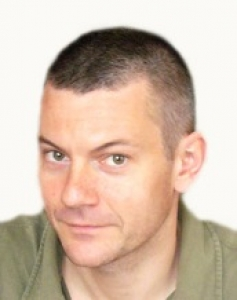
\includegraphics[width=1.6cm]{Stephane-Robin_inra_image.jpg} & 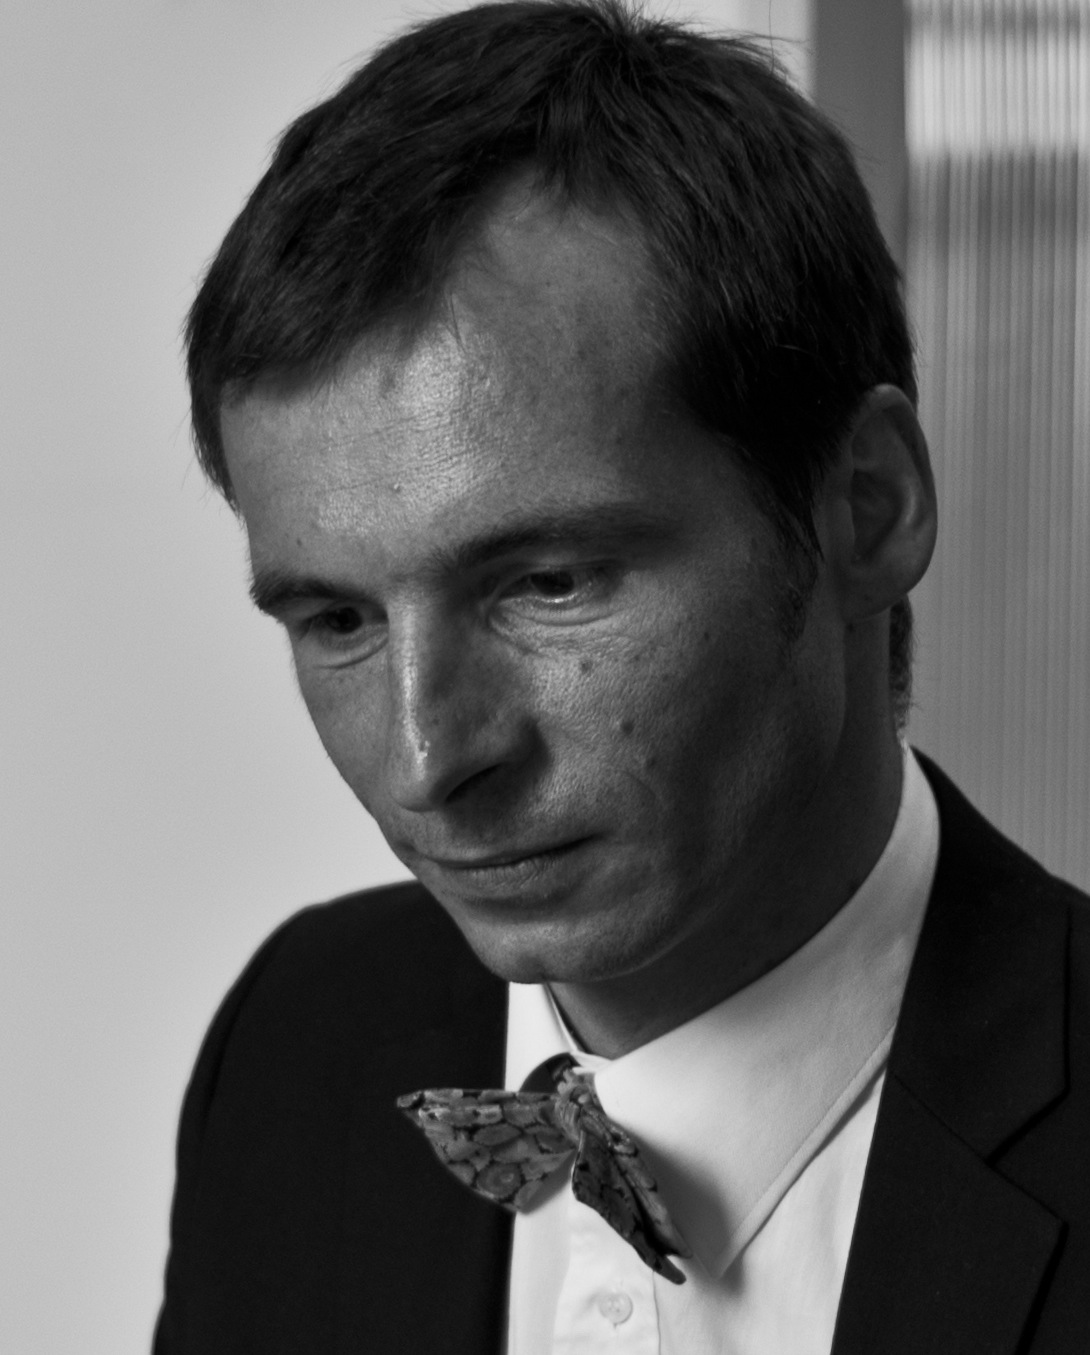
\includegraphics[width=1.6cm]{the-opponent.jpg}   \\
    \footnotesize{Stéphane Robin} &  \footnotesize{Chistophe Ambroise}
\end{tabular}
 
\end{center}
\item Supports:
    \begin{center}
	
\includegraphics[width=0.2\linewidth]{logo_inra.jpg}\hspace{0.15cm}
	
\includegraphics[width=0.2\linewidth]{agro.PNG}\hspace{0.1cm}
	
\includegraphics[width=0.2\linewidth]{lmh.png}\hspace{0.15cm}
	
\includegraphics[width=0.1\linewidth]{upsud.jpg}
    
\end{center}
\end{itemize}
\end{frame}

\section{Graphical models}
%%%%%%%%%%%%%%%%%%%%%%%%%%%%%%%%%%
%  GGM : matrice de précision encode la structure de dépendence
\subsection{Classical}
\begin{frame}{Statistical framework for conditional dependence}
\bleu{Example}:\bigskip
\begin{columns}
\begin{column}{0.3\linewidth}\hspace{0.5cm}
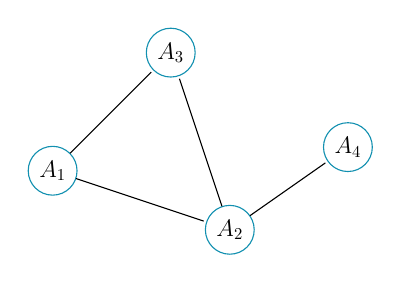
\begin{tikzpicture}	

      \tikzstyle{every edge}=[-,>=stealth',shorten >=1pt,auto,thin,draw]
		\node[observed] (A1) at (0*\edgeunit, 0*\edgeunit) {$A_1$};
		\node[observed] (A2) at (1.5*\edgeunit, -0.5*\edgeunit) {$A_2$};
		\node[observed] (A3) at (1*\edgeunit, 1*\edgeunit) {$A_3$};
		\node[observed] (A4) at (2.5*\edgeunit, 0.2*\edgeunit) {$A_4$};
		\path (A1) edge [] (A2)
        (A1) edge [] (A3)
        (A2) edge [] (A3)
        (A2) edge [] (A4);
	\end{tikzpicture}\\
\end{column}
\begin{column}{0.5\linewidth}
	\begin{itemize}
	\item Connected: all variables are dependant \bigskip
	\item \emphase{Markov property} : G encodes the conditional independences\\\bigskip
	 e.g. $A_4 \independent (A_1, A_3) \: |A_2$ \vspace{0.2cm}
\end{itemize}
\end{column}
\end{columns}
\begin{center}
 \only<1>{   \[ p(A_1, \dots, A_p) \propto \prod_{C \in \Ccal_G} \psi_C(A_C) \]
  where $\Ccal_G =$ set of maximal cliques of $G$.}
  \only<2>{ Here:  \[ P(A) \propto \psi_{1}(A_1,A_2,A_3) \; \psi_{2}(A_2,A_4) \]}
\end{center}
\end{frame}

%%%%%%%%%%%%%%%%%%%%%%%%%%%%%%%%%%
\begin{frame}{\textit{Gaussian Graphical Models} (GGM)}

The Gaussian setting gives the cliques directly.\bigskip\\
\only<1>{
$Y$ a multivariate Gaussian of dimension $d$:
\vspace{0.3cm}
\begin{center}
  $Y=(Y_1,...,Y_d) \sim \mathcal{N}_d(0,\Omega^{-1})$,\\
$\Omega  = (\omega_{ij})_{ i,j }$. \\
\end{center}
 \vspace{0.3cm}
 The factorization is straightforward:
\begin{align*}
p(y) &\propto exp(-y^T \Omega y /2)\\
&\propto \prod_{j,k : \emphase{\omega_{jk} \neq 0 }} exp(-y_j \omega_{jk} y_k /2)  
\end{align*}
}
\only<2>{
 \begin{columns} 
 \begin{column}{0.5\linewidth}

 \begin{flushright}
\[\Omega=
\left(
\begin{array}{*{4}{c}}
* & * & * & 0\\
*& * & * & *\\
* & * & * & 0\\
0 & * & 0 & *
\end{array}
\right)
\]
 \end{flushright}
 \end{column}
 \begin{column}{0.05\linewidth}
\begin{center}
 $\Rightarrow$
\end{center}
\end{column}
 \begin{column}{0.45\linewidth}
 \begin{flushleft}
\vspace{0.8cm}
 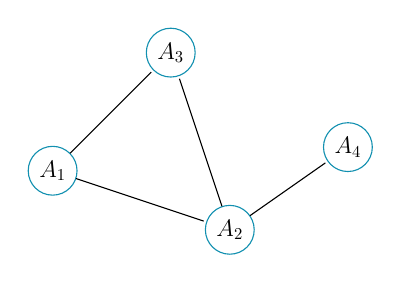
\begin{tikzpicture}
     
      \tikzstyle{every edge}=[-,>=stealth',shorten >=1pt,auto,thin,draw]
		\node[observed] (A1) at (0*\edgeunit, 0*\edgeunit) {$A_1$};
		\node[observed] (A2) at (1.5*\edgeunit, -0.5*\edgeunit) {$A_2$};
		\node[observed] (A3) at (1*\edgeunit, 1*\edgeunit) {$A_3$};
		\node[observed] (A4) at (2.5*\edgeunit, 0.2*\edgeunit) {$A_4$};
		\path (A1) edge [] (A2)
        (A1) edge [] (A3)
        (A2) edge [] (A3)
        (A2) edge [] (A4);

\end{tikzpicture}\\
\end{flushleft}
 \end{column}

\end{columns}}
\end{frame}

%%%%%%%%%%%%%%%%%%%%%%%%%%%%%%%%%%
% glasso : pénalisation donc parcimonie

\begin{frame}{Classical graph inference: the graphical Lasso}

 $Y$  log-likelihood:
 \[L(Y,\Omega) = \frac{n}{2}\log(det(\Omega))-\frac{n}{2} Y^T\Omega Y + cste\]

\bleu{Graphical-Lasso (glasso) :}
 
  \[\bleu{\widehat{\Omega}_\lambda }= \arg\min_{\Omega \in \mathcal{S}_d^+}\left\{ L(Y,\Omega)+\lambda \sum_{i\neq j} |w_{ij}| \right\}\]
\begin{itemize}
\item Sparse approach
\item Depends on a penalty  $\lambda$ (choice of grid, choice of  $\lambda^*$)
\end{itemize}
\end{frame}
%%%%%%%%%%%%%%%%%%%%%%%%%%%%%%%%%%
\subsection{Using trees}
%%%%%%%%%%%%%%%%%%%%%%%%%%%%%%%%%%
\begin{frame}{Mixture of trees: sparse and efficient}
\center{\emphase{Assumption : the underlying structure is a tree.}}

\bigskip

 \begin{description}
\item[Sparse structures: ]\begin{itemize}
\item[]
\end{itemize}
\emphase{$\text{\#} \mathcal{G}_p = 2^{\frac{p(p-1)}{2}}$}  reduced to  \emphase{$\text{\#} \mathcal{T}_p = p^{(p-2)}$}\bigskip\bigskip 

	\item[Suitable algebraic tool: ]\begin{itemize}
\item[]
\end{itemize}
Matrix tree theorem \citep{matrixtree}
$$\emphase{ \sum_{T\in \mathcal{T}}}\prod_{(k,l) \in T} \psi_{k,l}(Y)    \rightarrow \emphase{\mathcal{O} (p^3)}$$
\end{description}
%\vskip 
\center{
\textbf{Approach}: infer the network by \emphase{averaging spanning trees}}
\end{frame}
%====================================================================
%====================================================================

\begin{frame}{Concept of tree averaging} 
\begin{center}
    

%\begin{tabular}{p{\linewidth}}
%\begin{tabularx}{\linewidth}{ccccl}
 \begin{tabular}{ccccl}
   \begin{tabular}{c}
	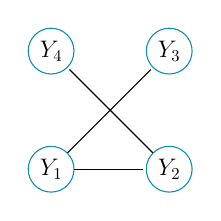
\begin{tikzpicture}
		
      \tikzstyle{every edge}=[-,>=stealth',shorten >=1pt,auto,thin,draw]
    
		\node[observed] (Z1) at (0*\edgeunit, 0*\edgeunit) {$Y_1$};
		\node[observed] (Z2) at (1*\edgeunit, 0*\edgeunit) {$Y_2$};
		\node[observed] (Z3) at (1*\edgeunit, 1*\edgeunit) {$Y_3$};
		\node[observed] (Z4) at (0*\edgeunit, 1*\edgeunit) {$Y_4$};
		\path (Z1) edge [] (Z2)
        (Z1) edge [] (Z3)
        (Z2) edge [] (Z4);
   
	\end{tikzpicture}\\
	\footnotesize{$P\{T = t_1 | Y\}$}
	   \end{tabular}
	   & 
	   \hspace{-.05\textwidth}% \pause
	   \begin{tabular}{c}
		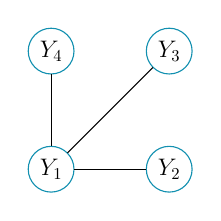
\begin{tikzpicture}
		\tikzstyle{every observed}=[draw=none,text=black,scale=0.5,
      transform shape,circular drop shadow] 
		\node[observed] (Z1) at (0*\edgeunit, 0*\edgeunit) {$Y_1$};
		\node[observed] (Z2) at (1*\edgeunit, 0*\edgeunit) {$Y_2$};
		\node[observed] (Z3) at (1*\edgeunit, 1*\edgeunit) {$Y_3$};
		\node[observed] (Z4) at (0*\edgeunit, 1*\edgeunit) {$Y_4$};
		
		\path (Z1) edge [] (Z2)
        (Z1) edge [] (Z3)
        (Z1) edge [] (Z4);
		\end{tikzpicture} \\
		\footnotesize{$P\{T = t_2 | Y\}$}
	   \end{tabular}
	   &
	   \hspace{-.05\textwidth} %\pause
	   \begin{tabular}{c}
		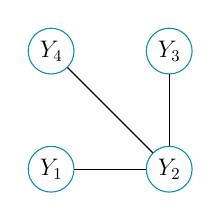
\begin{tikzpicture}
		\tikzstyle{every observed}=[draw=none,text=black,scale=0.5,
      transform shape,circular drop shadow] 
		\node[observed] (Z1) at (0*\edgeunit, 0*\edgeunit) {$Y_1$};
		\node[observed] (Z2) at (1*\edgeunit, 0*\edgeunit) {$Y_2$};
		\node[observed] (Z3) at (1*\edgeunit, 1*\edgeunit) {$Y_3$};
		\node[observed] (Z4) at (0*\edgeunit, 1*\edgeunit) {$Y_4$};
		
		\path (Z1) edge [] (Z2)
        (Z2) edge [] (Z3)
        (Z2) edge [] (Z4); 
		\end{tikzpicture}\\
		\footnotesize{$P\{T = t_3 | Y\}$}
	   \end{tabular}
	   &
	   \hspace{-.05\textwidth}% \pause
	   \begin{tabular}{c}
		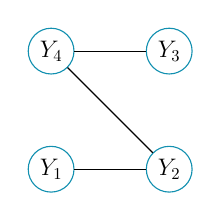
\begin{tikzpicture}
		\tikzstyle{every observed}=[draw=none,text=black,scale=0.5,
      transform shape,circular drop shadow] 
		\node[observed] (Z1) at (0*\edgeunit, 0*\edgeunit) {$Y_1$};
		\node[observed] (Z2) at (1*\edgeunit, 0*\edgeunit) {$Y_2$};
		\node[observed] (Z3) at (1*\edgeunit, 1*\edgeunit) {$Y_3$};
		\node[observed] (Z4) at (0*\edgeunit, 1*\edgeunit) {$Y_4$};
		 
		\path (Z1) edge [] (Z2)
        (Z3) edge [] (Z4)
        (Z2) edge [] (Z4);
		\end{tikzpicture} \\
		\footnotesize{$P\{T = t_4 | Y\}$}
	   \end{tabular}
	   & \hspace{-.06\textwidth} 
	   \huge{\emphase{...}}\normalsize   \\ \\
	   \\% \pause
	   \begin{tabular}{l}
		Compute edge\\
		probabilities:
	   \end{tabular}
	   &
	   \hspace{-.05\textwidth}
	   \begin{tabular}{c}
		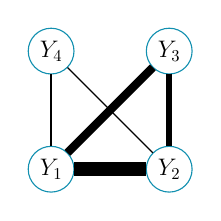
\begin{tikzpicture}
		\node[observed] (Z1) at (0*\edgeunit, 0*\edgeunit) {$Y_1$};
		\node[observed] (Z2) at (1*\edgeunit, 0*\edgeunit) {$Y_2$};
		\node[observed] (Z3) at (1*\edgeunit, 1*\edgeunit) {$Y_3$};
		\node[observed] (Z4) at (0*\edgeunit, 1*\edgeunit) {$Y_4$};
		\draw [line width=5pt] (Z1) -- (Z2); 
		\draw [line width=3pt] (Z1) -- (Z3); 
		\draw [line width=.5pt] (Z1) -- (Z4); 
		\draw [line width=2pt] (Z2) -- (Z3); 
		\draw [line width=.5pt] (Z2) -- (Z4); 
 %		\draw [line width=.5pt] (Z3) -- (Z4); 
		\end{tikzpicture}\\
		\emphase{$P\{(j, k) \in T | Y\}$}
	   \end{tabular}
	   &
	  \hspace{-.05\textwidth} %\pause
	   \begin{tabular}{l}
		Thresholding\\
		probabilities:
	   \end{tabular}
	   &
	   \hspace{-.05\textwidth}
	   \begin{tabular}{c}
		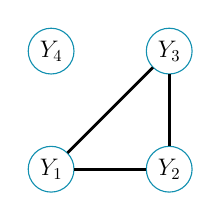
\begin{tikzpicture}
		\node[observed] (Z1) at (0*\edgeunit, 0*\edgeunit) {$Y_1$};
		\node[observed] (Z2) at (1*\edgeunit, 0*\edgeunit) {$Y_2$};
		\node[observed] (Z3) at (1*\edgeunit, 1*\edgeunit) {$Y_3$};
		\node[observed] (Z4) at (0*\edgeunit, 1*\edgeunit) {$Y_4$};
		\draw [line width=1pt] (Z1) -- (Z2); 
		\draw [line width=1pt] (Z1) -- (Z3); 
% 		\draw [line width=1pt] (Z1) -- (Z4); 
		\draw [line width=1pt] (Z2) -- (Z3); 
% 		\draw [line width=.1pt] (Z2) -- (Z4); 
% 		\draw [line width=1pt] (Z3) -- (Z4); 
		\end{tikzpicture}
	   \end{tabular}
	   &
	 \end{tabular}
   % \end{tabular}
   %\end{tabularx}
   \end{center}
\end{frame}

%$T \sim \prod_{jk}\beta_{jk}/B$

%%%%%%%%%%%%%%%%%%%%%%%%%%%%%%%%%%
% arbre : structure
\section{Model for Gaussian data}
\subsection{tree-based GM}
\begin{frame}{Spanning tree structure}
Acyclic graph connecting all the nodes\\
\begin{table}[]
\begin{tabular}{ll|l|l}
\multicolumn{2}{c|}{spanning trees} & not spanning & not a tree \\
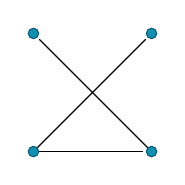
\begin{tikzpicture}	
      \tikzstyle{every edge}=[-,>=stealth',shorten >=1pt,auto,thin,draw]
    
		\node[basic] (Z1) at (0*\edgeunit, 0*\edgeunit) {};
		\node[basic] (Z2) at (1*\edgeunit, 0*\edgeunit) {};
		\node[basic] (Z3) at (1*\edgeunit, 1*\edgeunit) {};
		\node[basic] (Z4) at (0*\edgeunit, 1*\edgeunit) {};
		\path (Z1) edge [] (Z2)
        (Z1) edge [] (Z3)
        (Z2) edge [] (Z4);
	\end{tikzpicture} & 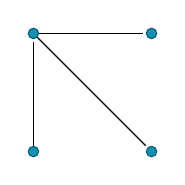
\begin{tikzpicture}	
      \tikzstyle{every edge}=[-,>=stealth',shorten >=1pt,auto,thin,draw]
    
		\node[basic] (Z1) at (0*\edgeunit, 0*\edgeunit) {};
		\node[basic] (Z2) at (1*\edgeunit, 0*\edgeunit) {};
		\node[basic] (Z3) at (1*\edgeunit, 1*\edgeunit) {};
		\node[basic] (Z4) at (0*\edgeunit, 1*\edgeunit) {};
		\path (Z1) edge [] (Z4)
        (Z4) edge [] (Z2)
        (Z4) edge [] (Z3);
	\end{tikzpicture} &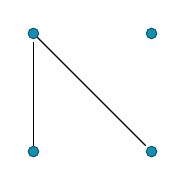
\begin{tikzpicture}	
      \tikzstyle{every edge}=[-,>=stealth',shorten >=1pt,auto,thin,draw]
    
		\node[basic] (Z1) at (0*\edgeunit, 0*\edgeunit) {};
		\node[basic] (Z2) at (1*\edgeunit, 0*\edgeunit) {};
		\node[basic] (Z3) at (1*\edgeunit, 1*\edgeunit) {};
		\node[basic] (Z4) at (0*\edgeunit, 1*\edgeunit) {};
		\path (Z1) edge [] (Z4)
        (Z4) edge [] (Z2) ;
	\end{tikzpicture}  & 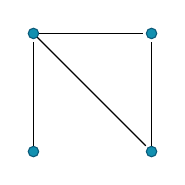
\begin{tikzpicture}	
      \tikzstyle{every edge}=[-,>=stealth',shorten >=1pt,auto,thin,draw]
    
		\node[basic] (Z1) at (0*\edgeunit, 0*\edgeunit) {};
		\node[basic] (Z2) at (1*\edgeunit, 0*\edgeunit) {};
		\node[basic] (Z3) at (1*\edgeunit, 1*\edgeunit) {};
		\node[basic] (Z4) at (0*\edgeunit, 1*\edgeunit) {};
		\path (Z1) edge [] (Z4)
        (Z4) edge [] (Z2)
        (Z4) edge [] (Z3)
        (Z2) edge [] (Z3);
	\end{tikzpicture}
\end{tabular}
\end{table}
\begin{itemize}
\item all variables are dependent, few are conditionally dependent 
\item cliques are edges : \emphase{Tree-based graphical model}:$$p(Y|T) \propto \prod_{jk \in T} \psi_{jk}(Y_j,Y_k)$$ if p is faithful to the spanning tree T.
\end{itemize}

\end{frame}
%%%%%%%%%%%%%%%%%%%%%%%%%%%%%%%%%%

% modèle de mélange d'arbres meila : loi décomposable sur les arêtes
\begin{frame}{Distribution over tree structures}
\cite{MeilaJaak}: decomposable distribution defined by a set of \emphase{weights} $\left\{\beta_{jk}, jk \in T\right\}$
$$p(T) = \frac{1}{B}\prod_{jk\in T}\beta_{jk}$$
Where B is the normalization constant : $B = \sum_{T \in \mathcal{T} } \prod_{jk} \beta_{jk} $
\bigskip
\begin{itemize}
\item An edge contributes the same amount in every tree that includes it
\item The probability of a tree $\propto$ the product of its edges weights
\end{itemize}
\end{frame}


%%%%%%%%%%%%%%%%%%%%%%%%%%%%%%%%%%

%%%%%%%%%%%%%%%%%%%%%%%%%%%%%%%%%%
\begin{frame}{Tree-based mixture}
Each sample $i$ of $Y$ is a mixture on tree-shaped structures (\cite{MeilaJaak},\cite{kirshner}):
\begin{align*}
\{Y_{i.}\}_i & \independent | \:T \\
p(Y_{i.})& = \sum_{T\in\mathcal{T}}p(T)p(Y_{i.}|T) 
\end{align*}

Marginal distribution :
$$ p(Y_{i.}) \propto \sum_{T\in\mathcal{T}} \prod_{jk\in T} \beta_{jk} \psi_{jk}(Y_{ij},Y_{ik})$$
\end{frame}
%%%%%%%%%%%%%%%%%%%%%%%%%%%%%%%%%%

\begin{frame}{Tree-based mixture model with Gaussian data}
$$p(T) = \frac{1}{B}\prod_{jk\in T}\beta_{jk} \;\; ; \;\;B = \sum_{T \in \mathcal{T} } \prod_{jk} \beta_{jk} $$
$$p(Y|T) \propto \prod_{jk \in T} \psi_{jk}(Y)$$ 
$$ p(Y) \propto \sum_{T\in\mathcal{T}} \prod_{jk\in T} \beta_{jk} \psi_{jk}(Y)$$
\end{frame}
%%%%%%%%%%%%%%%%%%%%%%%%%%%%%%%%%%
\subsection{Algebraic tool}
\begin{frame}{Matrix-tree theorem}
\emphase{Theorem} \citep{matrixtree} Let $W=[w_{jk}] $be a matrix with null diagonal and $\Delta(W)$ its Laplacian :
$$\Delta=\left\{ 
					\begin{array}{ll}
						\sum_k w_{jk}& \text{ if } j=k\\
						-w_{jk} & \text{otherwise }
					\end{array}
				\right.$$
Then all cofactors $|\Delta(W)|^{uv} $ are equal and
$$ |\Delta(W)|^{uv} = \sum_{T\in\mathcal{T}}\prod_{jk \in T} w_{jk} $$

\emphase{Corollary} Denote $W^{ab}$ the same matrix but setting $w_{ab}=w_{ba}=0$:
$$  |\Delta(W^{ab})|^{ab}  = \sum_{T\in\mathcal{T}:ab\notin T}\prod_{jk\in T} w_{jk}$$
\end{frame}
%%%%%%%%%%%%%%%%%%%%%%%%%%%%%%%%%%
\section{Inference}
\subsection{Procedure}
\begin{frame}{EM algorithm}
T is a latent variable. The complete log-likelihood is:
$$ \log(p(\emphase{T},Y)) = \sum_{j,k} \mathds{1}\{jk \in T\} \left( \log \emphase{\beta_{jk}} + \sum_i \log \psi_{jk}(Y)\right) - \log \emphase{B}$$
Objective function of EM:
$$\mathds{E}\left[\log(p(\emphase{T},Y)|Y\right]) = \sum_{j,k} \mathds{P}\{jk\in T |Y\}\left( \log \emphase{\beta_{jk}} + \sum_i \log \psi_{jk}(Y)\right) - \log \emphase{B}$$
\end{frame}
%%%%%%%%%%%%%%%%%%%%%%%%%%%%%%%%%%
\begin{frame}{EM algorithm: E step}
Compute $\mathds{P}\{jk\in T |Y\}$ and B thanks to the matrix-tree theorem and corollary:

$$\emphase{B = |\Delta([\beta_{jk}])|^{11}}$$
\begin{align*}
\mathds{P}\{jk\in T |Y\} &= \sum_{T\in \mathcal{T}: jk\in T} p(T|Y)\\
&=\sum_{T\in \mathcal{T}: jk\in T} \frac{p(T)p(Y|T)}{p(Y)}\\
\emphase{P_{jk}}&\emphase{=1-\frac{|\Delta([\beta\psi]^{jk})|^{jk}}{|\Delta([\beta\psi])|^{11}}}
\end{align*}

\end{frame}
%%%%%%%%%%%%%%%%%%%%%%%%%%%%%%%%%%
 \begin{frame}{EM algorithm: M step}

\[\hat{\beta}_{jk} = \argmax_{\beta_{jk}} \left\{\sum_{j,k} P_{jk}\left( \log \emphase{\beta_{jk}} + \sum_i \log \psi_{jk}(Y)\right) - \log \emphase{B}\right\}\]
\bigskip\bigskip
\[ \frac{\partial\mathds{E}_\theta[\log(p(Y,T))|Y]}{\partial\beta_{jk}} =\frac{ P_{jk} }{\beta_{jk}} - \frac{1}{B}
\emphase{\partial_{\beta_{jk}} B}
\]
 
\end{frame}
%%%%%%%%%%%%%%%%%%%%%%%%%%%%%%%%%%

 \begin{frame}{EM algorithm: M step}

\emphase{Lemma}  \citep{MeilaJaak}:\\
\footnotesize
    Define the entries of the symmetric matrix $M$ as

\[    
 [M]_{jk}=\begin{cases}
    \left[(\Delta(W)^{pp})^{-1}\right]_{jj} + \left[(\Delta(W)^{pp})^{-1}\right]_{kk}    		-2\left[(\Delta(W)^{pp})^{-1}\right]_{jk} & 1\leq j<k < p\\
    \left[(\Delta(W)^{pp})^{-1}\right]_{jj} & k=p, 1\leq j \leq p  \\
    0 & 1\leq j=k \leq p.
    \end{cases}
\]
\normalsize
Then it holds that

$$
\partial_{w_{jk}} W = [M]_{jk} \times W.
$$

\bigskip\bigskip

Which gives the following closed form update for step (h+1):
\emphase{
   \large{\[\hat{\beta}_{jk}^{h+1} = \frac{P_{jk}^h}{M_{jk}^h}\]}
}
 \end{frame}

\subsection{Validation}
\begin{frame}{A valid approach}
\begin{center}
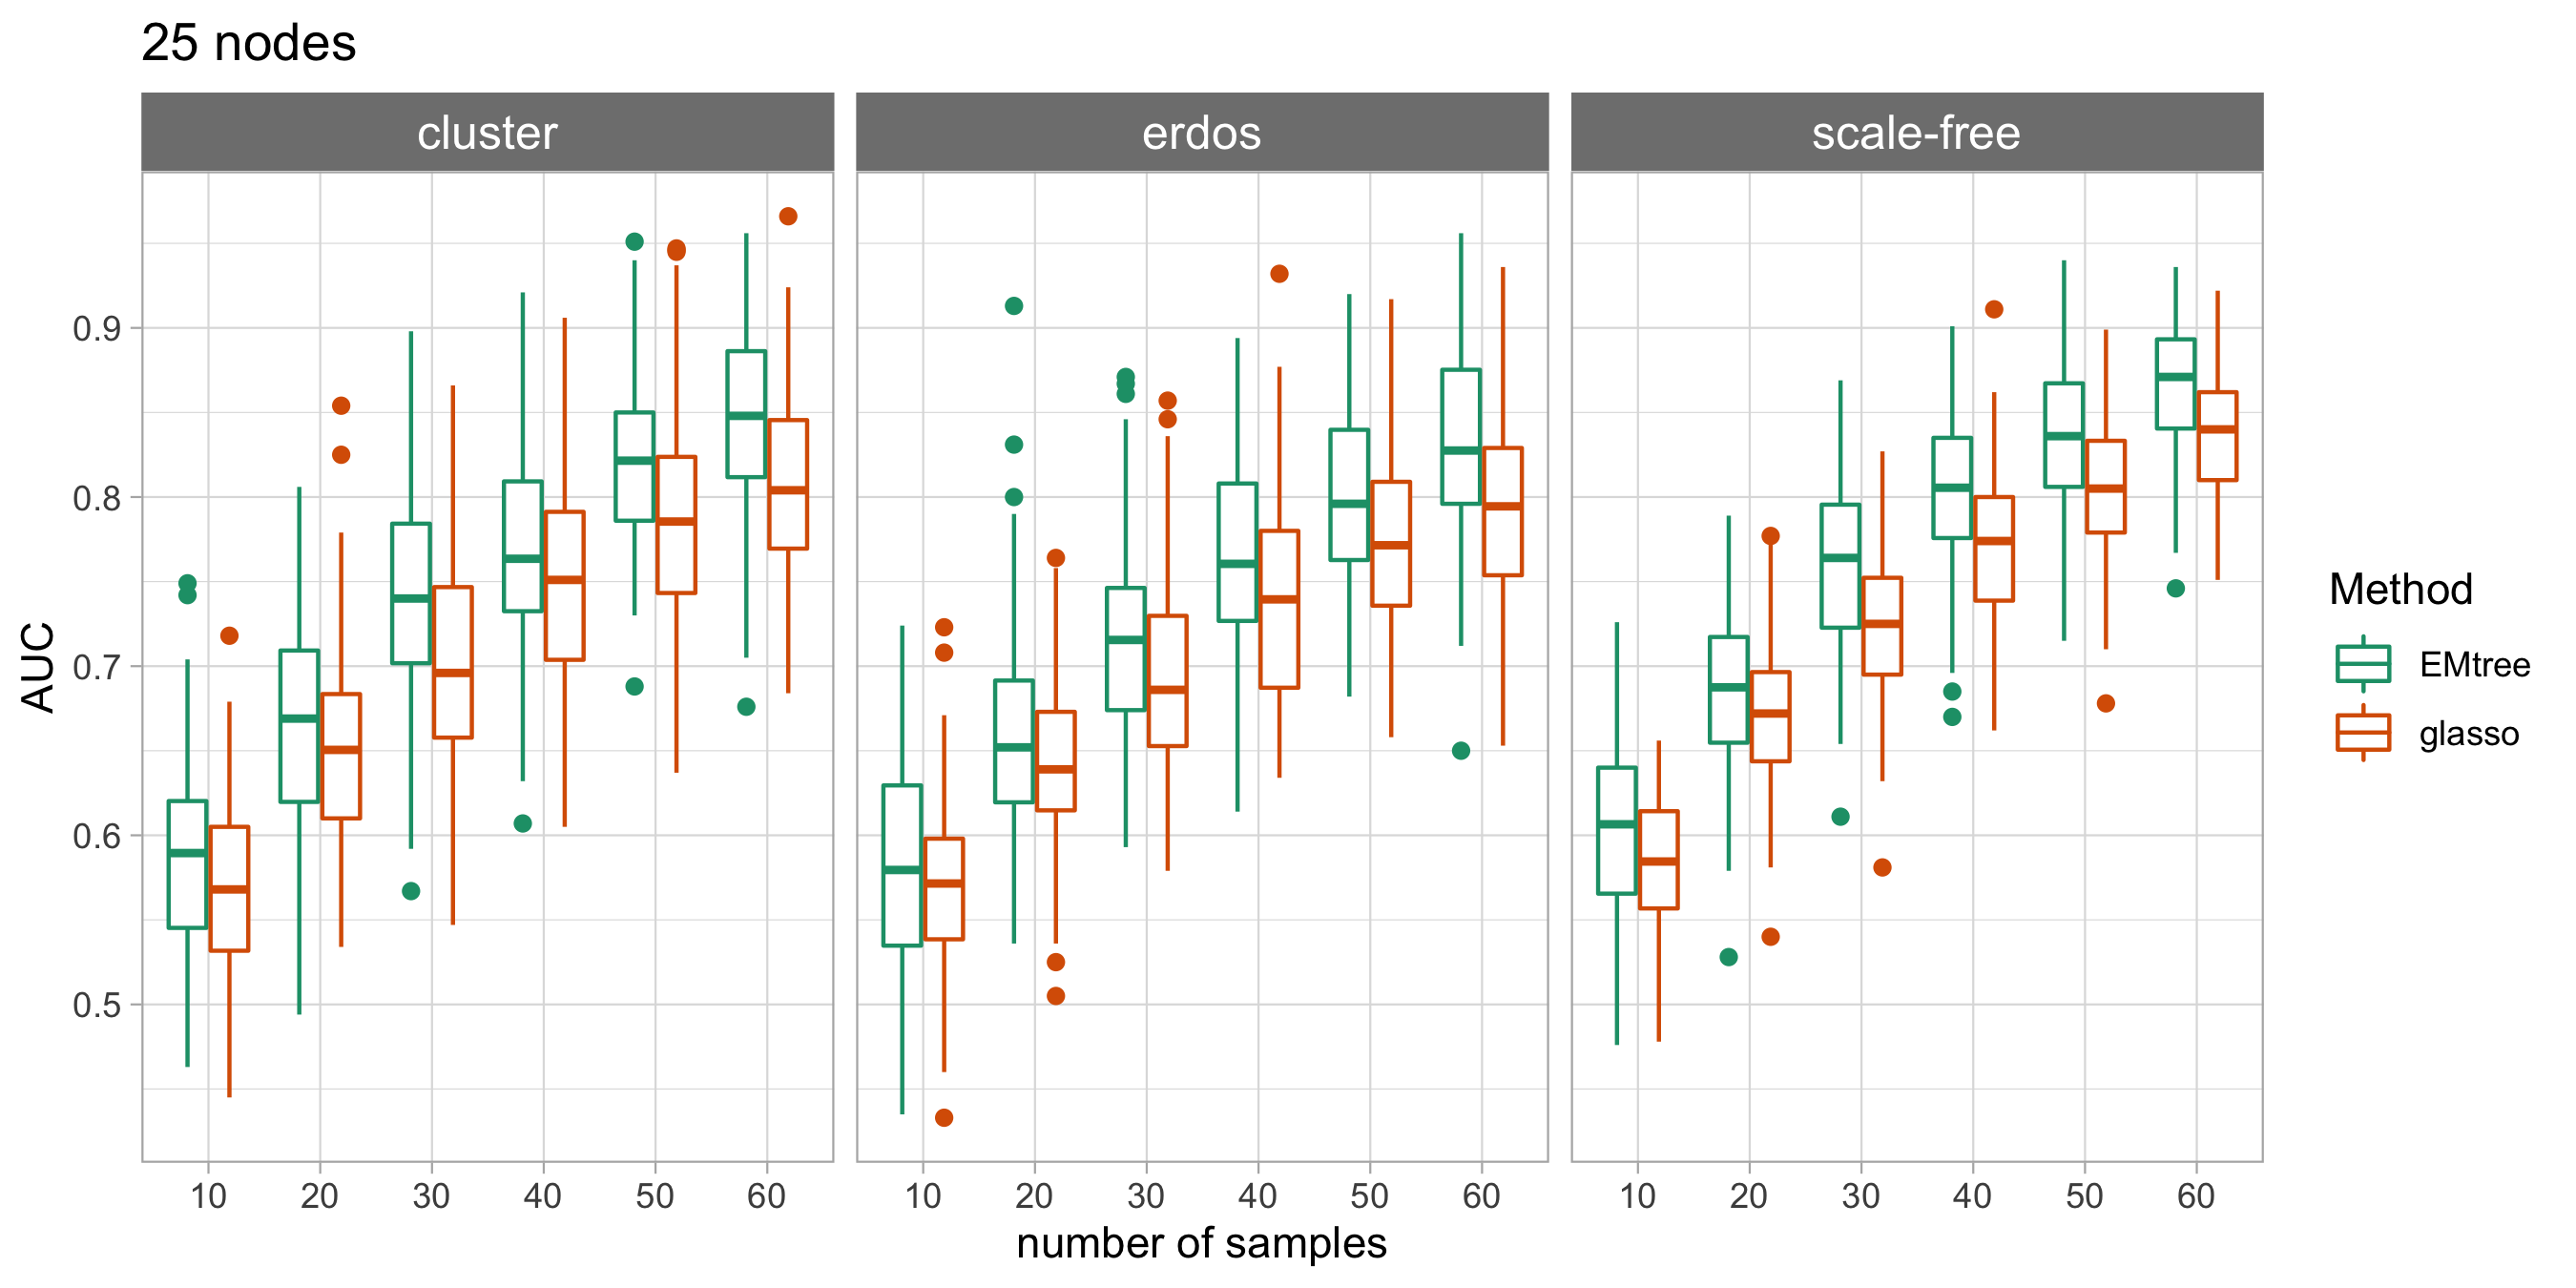
\includegraphics[width=11.5cm]{compare_glasso_penalty.png}
\end{center}
\footnotesize
Scores compared :
\begin{itemize}
\item EMtree: edges conditional probabilities.
\item glasso: maximal penalty under which an edge is included in the graph.
\end{itemize}
\end{frame}
%%%%%%%%%%%%%%%%%%%%%%%%%%%%%%%%%%
\section{}
\subsection{}

\begin{frame}
\center{\Huge\bleu{With abundance data}}
\end{frame}
%%%%%%%%%%%%%%%%%%%%%%%%%%%%%%%%%%
\section{Context}
\subsection{Abundance data}
\begin{frame}{Network example in ecology}
\begin{columns}

\begin{column}{7.5cm}
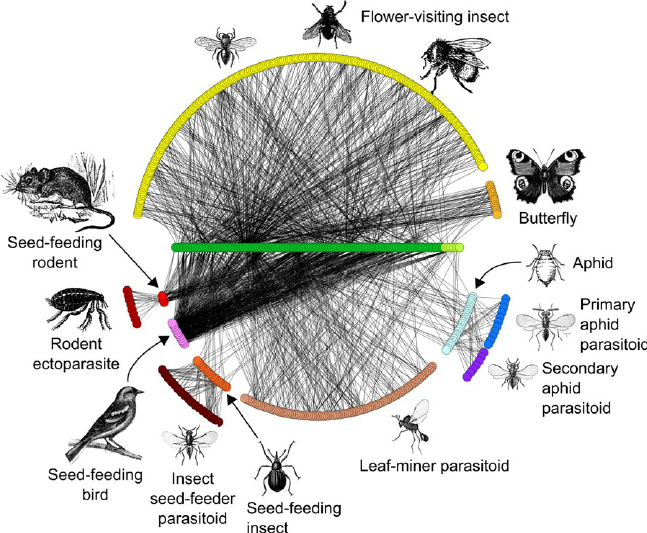
\includegraphics[width=8cm]{Species-interaction-networks-at-Norwood-Farm-Somerset-UK-revised-from-Pocock-et-al.png}

\footnotesize{Pocock et. al 2012}
\end{column}

\begin{column}{4.5cm}
\begin{itemize}
    \item Tool to better understand species interactions, eco-systems organizations
    \item Allows for resilience analyses, pathogens control, ecosystem comparison, response prediction...
\end{itemize}
\end{column}

\end{columns}
    
\end{frame}

\begin{frame}{Aim of network inference from abundance data}
    \begin{figure}[H]
   
    \begin{tabular}{lllll}
%        $\Xb$ & & $\Yb$ & & $\widehat{G}$ \\
        {\scriptsize{ \begin{tabular}{rr}
date & site \\
%\hline
apr93 & km03 \\
apr93 & km03 \\
apr93 & km03 \\
apr93 & km03 \\
apr93 & km17 \\
apr93 & km17 \\
\vdots & \vdots
\end{tabular} }} & \vspace{0.15cm} &
        {\tiny{ \begin{tabular}{rrrrr}
EFI & ELA & GDE & GME & HFA \\
%\hline
 71 &   1 &   5 &   6 &   0 \\
118 &   2 &   3 &   0 &   0 \\
 69 &   0 &   6 &   2 &   0 \\
 56 &   0 &   0 &   0 &   0 \\
  0 &   1 &   1 &   0 &   0 \\
  0 &   0 &   2 &   0 &   0 \\
\vdots & \vdots & \vdots & \vdots & \vdots
\end{tabular}
%
%\begin{tabular}{rrrrrrr}
%\dots & EFI & ELA & GDE & GME & HFA & \dots \\
%\hline
%&  71 &   1 &   5 &   6 &   0 & \\
%& 118 &   2 &   3 &   0 &   0 & \\
%&  69 &   0 &   6 &   2 &   0 & \\
%&  56 &   0 &   0 &   0 &   0 & \\
%&   0 &   1 &   1 &   0 &   0 & \\
%&   0 &   0 &   2 &   0 &   0 & \\
%& \vdots & \vdots & \vdots & \vdots & \vdots
%\end{tabular} }} & \vspace{0.15cm} &
        \begin{tabular}{c}
        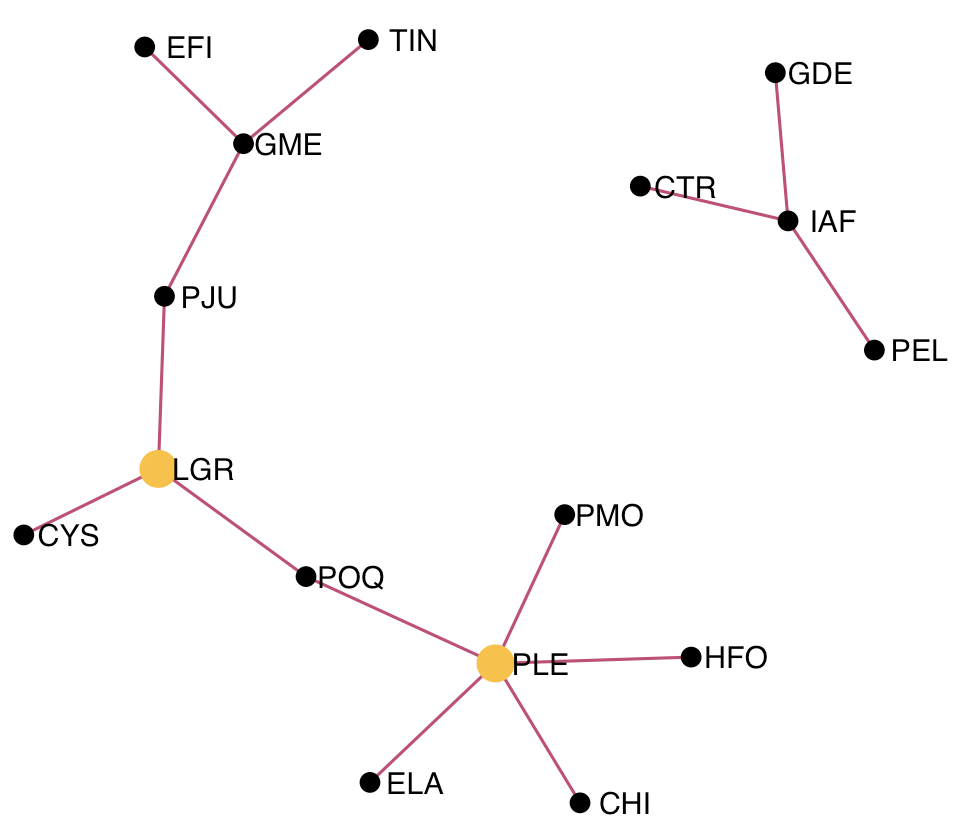
\includegraphics[width=.25\linewidth]{barans2plot.png}
        \end{tabular} \\
        ($a$) covariates $\bf{X}$ & & ($b$) species abundances $\bf{Y}$ & & ($c$) inferred network \\
    \end{tabular}
    \caption{Data sample from the Fatala river dataset (ade4 R package). }
    \label{fig:networkinference}
\end{figure}
\begin{itemize}
    \item Unknown underlying structure
    \item Unobserved interaction data 
\end{itemize}
\end{frame}


%====================================================================
%====================================================================

\section{Statistical modelling}

%====================================================================
%====================================================================


\subsection{The observed counts}

%====================================================================
%====================================================================
\begin{frame}{$P\ell N$ model }

   \Large{ $$ Y_{ij} \sim \mathcal{P}\left(\exp(o_{ij} + x_i^\intercal \thetab_j + Z_{ij})\right).$$} \normalsize
   \begin{itemize}
       \item A latent variable model
       \item easy handling of multi-variate data, offsets and covariates\\
   \end{itemize}
   \bigskip
   Random effects $Z$  add \emphase{dependence} among species. Classically \citep{AiH89}:
   $$ Z \sim\mathcal{N}(0,\Sigma)$$
   We  use  a mixture of tree structures:
   $$ Z \sim \sum_{T\in \mathcal{T}} p(T)\mathcal{N}(0,\Sigma_T), \hspace{1cm} T \sim \prod_{jk}\beta_{jk}/B $$
   
\end{frame}


\section{Inference}
%====================================================================
%====================================================================
\subsection{EM algorithm}


\begin{frame}{Direct EM algorithm ?}
\footnotesize 
\begin{itemize}
    \item \bleu{Complete likelihood :}

 \[ p(Y,Z,T) = \color{olive}p(T)\color{black}\times\color{blue}p(Z|T)\color{black}\times\color{orange}p(Y|Z)\]
 
\begin{align*}
 \log(\mathds{P}(Y,Z,T)) &= \sum_{k,l} \mathds{1}_{\{(k,l) \in T\}} \left[\color{olive}\log(\beta_{kl})\color{black} + \color{blue}\log(\psi_{kl}(Z)) \color{black}\right]-\color{olive}\log(B)\color{black} \\
 &+\sum_k \left[\color{blue} \log(p(Z_k))\color{black} + \color{orange}\log(p(Y_k|Z_k))\color{black}\right]
 \end{align*}

 \item \bleu{Conditional expectation :}
\end{itemize}
\begin{align*}
    \mathds{E}_\theta[\log(\mathds{P}(Y,Z,T))|Y] =&\sum_{k,l\in T} \mathds{P}((k,l) \in T|Y) \log(\beta_{kl}) + \mathds{E}[\mathds{1}_{\{(k,l) \in T\}}\emphase{\log(\psi_{kl}(Z)|Y)}]\\
& +\sum_k \emphase{\mathds{E}[\log(p(Z_k)) | Y]} + \mathds{E}[\log(p(Y_k|Z_k)) | Y]-\log(B)
\end{align*} 

\normalsize 
\end{frame}
\begin{frame}{Two hidden quantities}
Our model includes two hidden layers of parameters. We need to compute conditional probabilities:
 \bigskip
 
\begin{itemize}
    \item \emphase{$p(T|Y)$}: computationally complex but tractable thanks to the matrix-tree theorem and results from \bleu{ \cite{MeilaJaak}}.
    \bigskip
    \item \emphase{$p(Z|Y)$}: no close form, a VEM gives $\hat{\Sigma}$ and 
    $\hat{\theta}$ (VEM: \bleu{\citet{CMR17}}).
\end{itemize}
\end{frame}
%====================================================================
%====================================================================

%====================================================================
%====================================================================


\begin{frame}{EMtree algorithm}
\begin{description}
\item [Input: ] \hspace{0.35cm}Abundance data, covariates, offsets\vspace{0.2cm}

\item [1rst step: ] \hspace{0.3cm}VEM algorithm to \emphase{fit PLN model} $\Rightarrow$  $\hat{\theta}$, $\hat{\Sigma}_Z$. \vspace{0.2cm}
\item [2nd step: ] \hspace{0.3cm}EM algorithm to \emphase{update the $\beta_{jk}$} $\Rightarrow$ conditional probabilities for all edges.\\ 
\end{description}

 \only<1>{ \bigskip\bigskip
 $$Y_{ij} \sim \mathcal{P}\left(\exp(o_{ij} + x_i^\intercal \thetab_j + Z_{ij})\right).$$
  $$ Z \sim \sum p(T)\mathcal{N}(0,\Sigma_T), \hspace{1cm} T \sim \prod_{jk}\beta_{jk}/B $$}
\pause \bigskip
\begin{description}
\item [Thresholding: ] Select edges with probability above the probability of edges in a tree drawn uniformly (\emphase{$2/p$})\vspace{0.2cm}
\item [Resampling: ] \hspace{0.25cm}Strengthen the results: only edges selected in more than \emphase{$80\%$} of $S$ sub-samples are kept.
\end{description} \bigskip

\center{ \url{https://github.com/Rmomal/EMtree}}
\begin{figure}
    \centering
    
\includegraphics[width=0.6cm]{github.png}
\end{figure}
\end{frame}
\section{Application}
\subsection{Fatala River fishes}

\begin{frame}{Inferred networks: Fatala River fishes example}
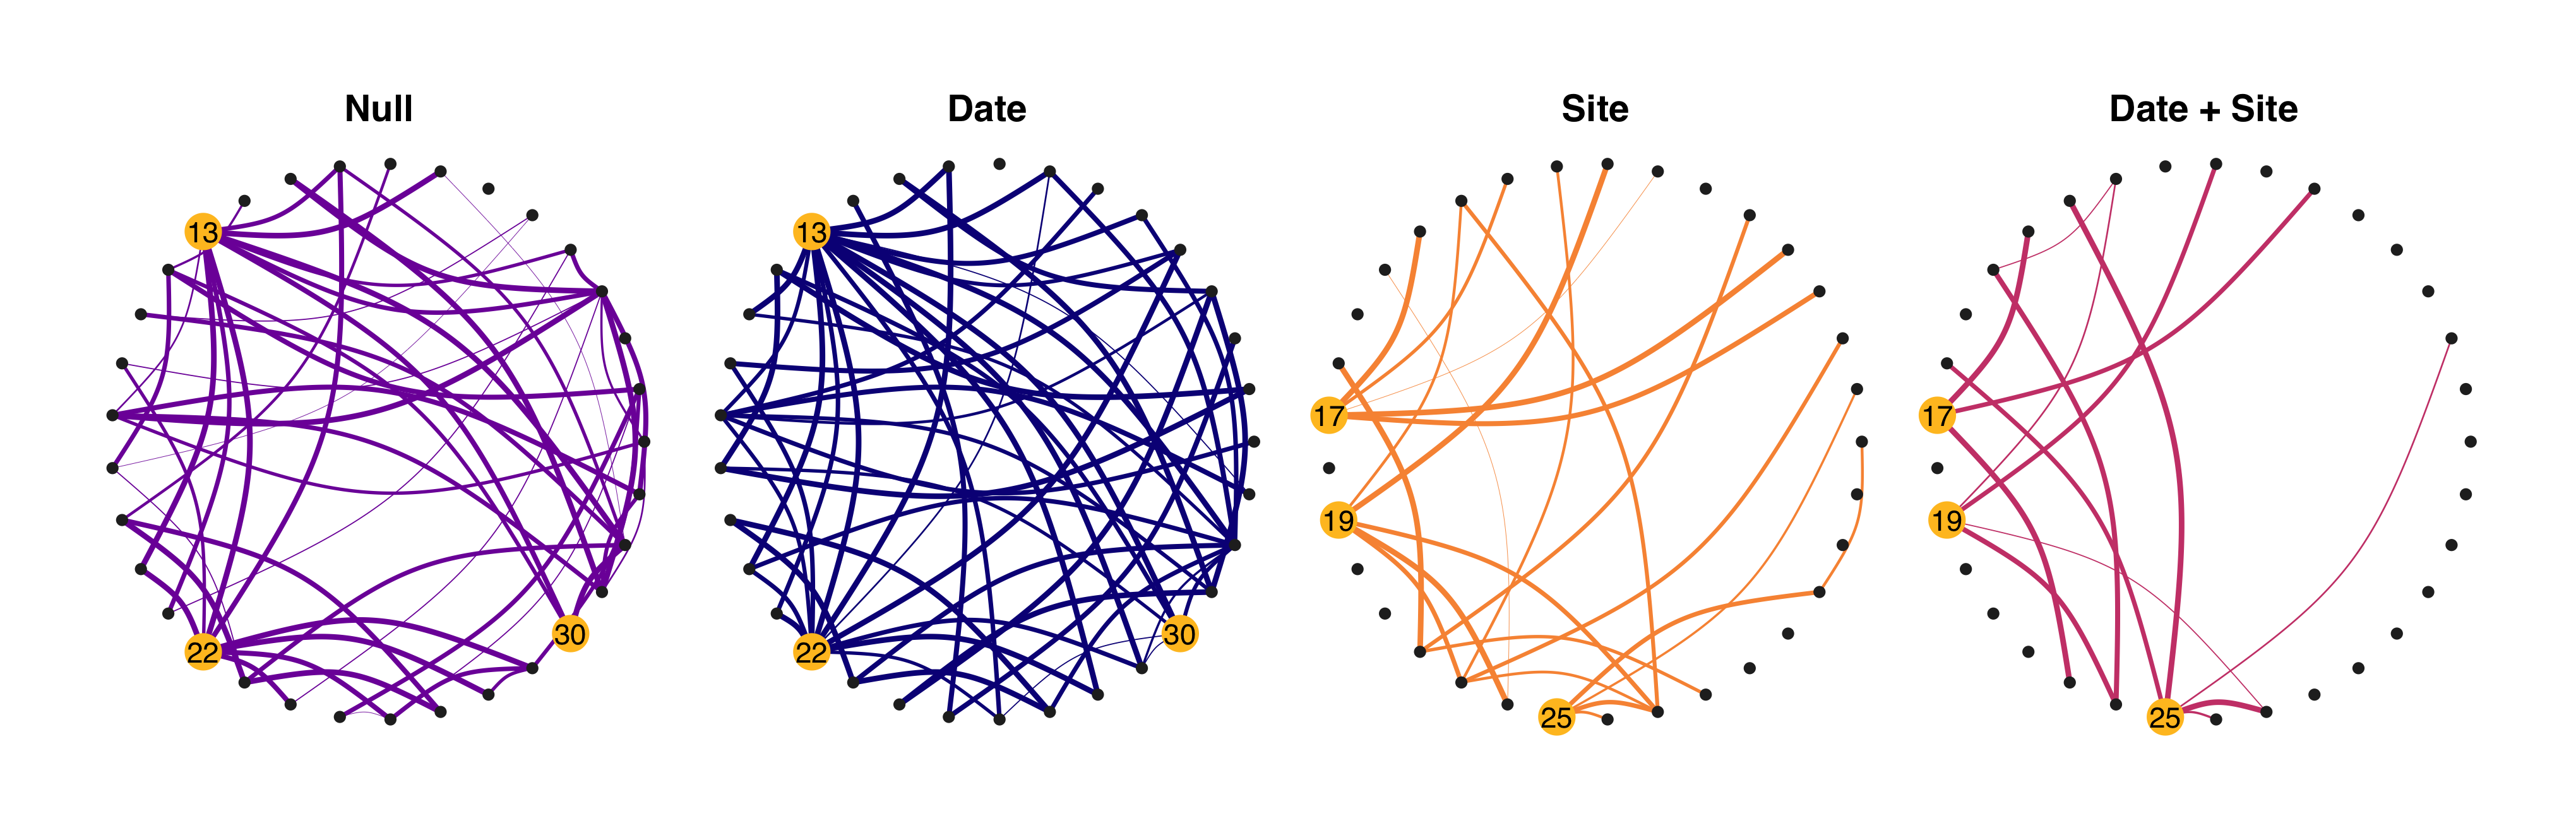
\includegraphics[width=\linewidth]{BaransNets.png}
\begin{itemize}
\item Dramatic effects of covariates on the structure
\item HIghlighted nodes: nodes with high betweenness scores
\end{itemize}
\end{frame}
\section{Evaluating performances}

\subsection{Simulation study}
%====================================================================
%====================================================================

\begin{frame}{Alternative approaches}

 Three  methods from microbiology:
    \begin{itemize}
        \item \emphase{SpiecEasi} algorithm \citep{kurtz} 
        \item \emphase{gCoda} \citep{gcoda} 
        \item \emphase{MInt} \citep{MInt} (uses PLN model)
    \end{itemize}\bigskip
    
  Two  methods from ecology:
  \begin{itemize}
  \item \emphase{ecoCopula}\citep{PWT19}
  \item \emphase{MRFcov}\citep{CWL18}
  \end{itemize}
  \bigskip
All rely on a GGM or a Gaussian copula, so that the network inference problem amounts to estimating a sparse version of the precision matrix.
\end{frame}


\begin{frame}{Simulation design}

\begin{enumerate}
     \item Choose  \emphase{$G$} and randomly define the sign of its entries
     \item build \emphase{$\Omega_G = \Delta(G) + \delta\times \text{I}$}, positive definite and   \emphase{$\Sigma_G = \Omega_G^{-1}$} accordingly
     \item Sample count data \emphase{$Y$} from $\mathcal{P\ell N}(X,\Sigma_G)$ 
     \item Infer the networks with all methods
     \item Compare results with  presence/absence of edges (\emphase{FDR}, \emphase{AUC})
\end{enumerate}

\end{frame}

%====================================================================
%====================================================================

\subsection{Results}
\begin{frame}{Difficulty level: Erdös results}
\footnotesize{\bleu{False Discovery Rate (FDR):} how many false edges there is among what is detected ?\\
\bleu{Density ratio:} number of detections over the number of true edges}

\begin{figure}
    \centering
       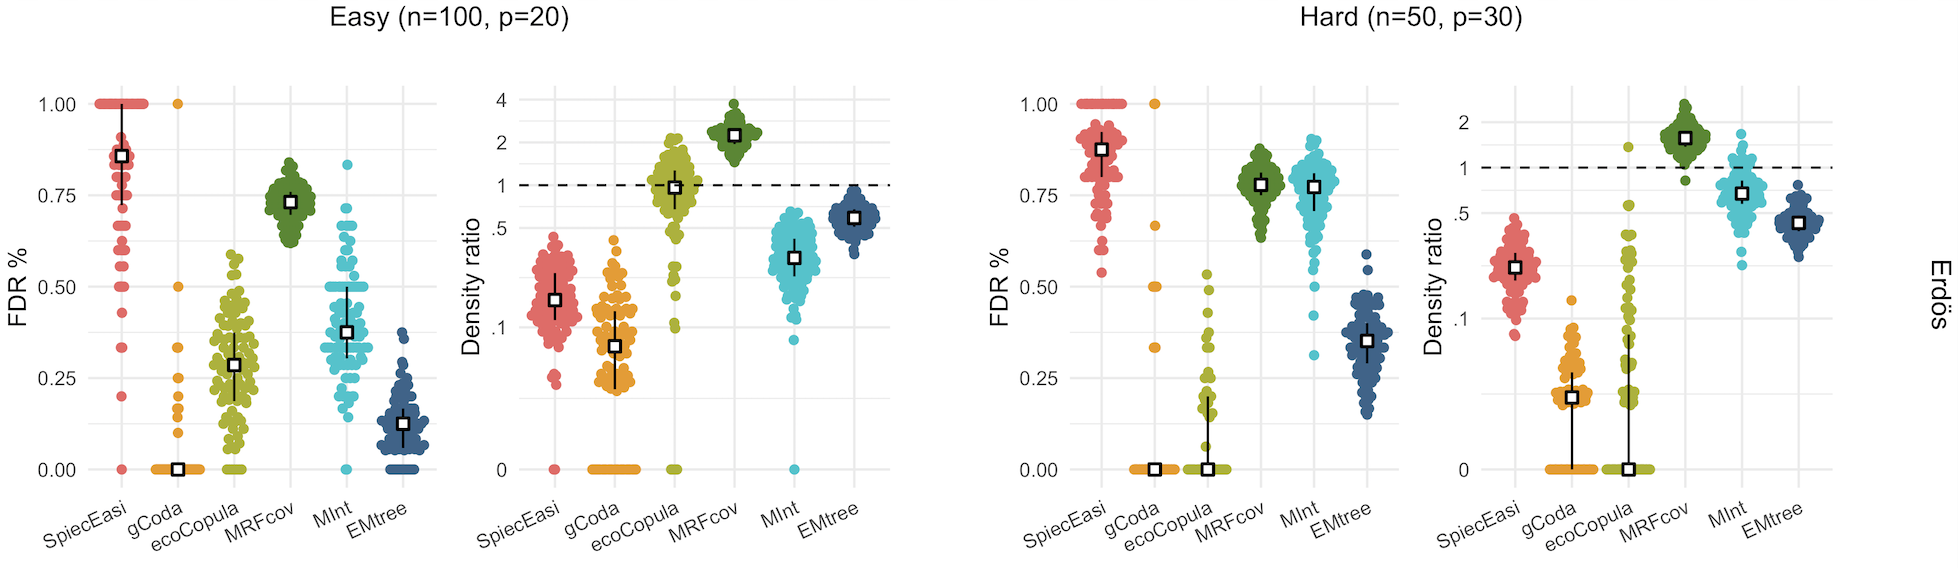
\includegraphics[width=\linewidth]{panelTPFN_signed_erdos} 
\end{figure}
\begin{itemize}
    \item EMtree: the smallest FDR with a reasonable density ratio
    \item The performance is maintained when increasing the difficulty level
\end{itemize}
\end{frame}
\begin{frame}{Difficulty level: running times}

\scriptsize
\begin{table}[ht]
\centering
\begin{tabular}{l|llllll}

 & SpiecEasi & gCoda & ecoCopula & MRFcov & MInt & EMtree \\ 
  \hline
Easy & 25.45(1.87) & 0.11(0.06) & 5.55(0.64) & 34.51(3.68) & 43.04(19.76) & 11.72(1.89) \\ 
  Hard & 28.43(1.3) & 0.53(0.25) & 9.6(0.65) & 8.29(0.36) & 33.77(18.2) & 8.17(0.5) \\ 
   \hline
\end{tabular}
\caption{Median and standard-deviation running-time values (in seconds) for Cluster and Erdös structures, including resampling with $S=20$ for SpiecEasi and EMtree.}
\label{timesTPFN}
\end{table}
\normalsize
\begin{itemize}
\item EMtree ranks $3^{rd}$/6 in easy cases and $2^{nd}$ in hard ones 
\end{itemize}
\end{frame}
\begin{frame}{Network density}
\footnotesize{\bleu{Area under the (ROC) curve (AUC):} "how good is a classifier to rank true positives higher"}\\
 \begin{figure}[H]
  \centering
  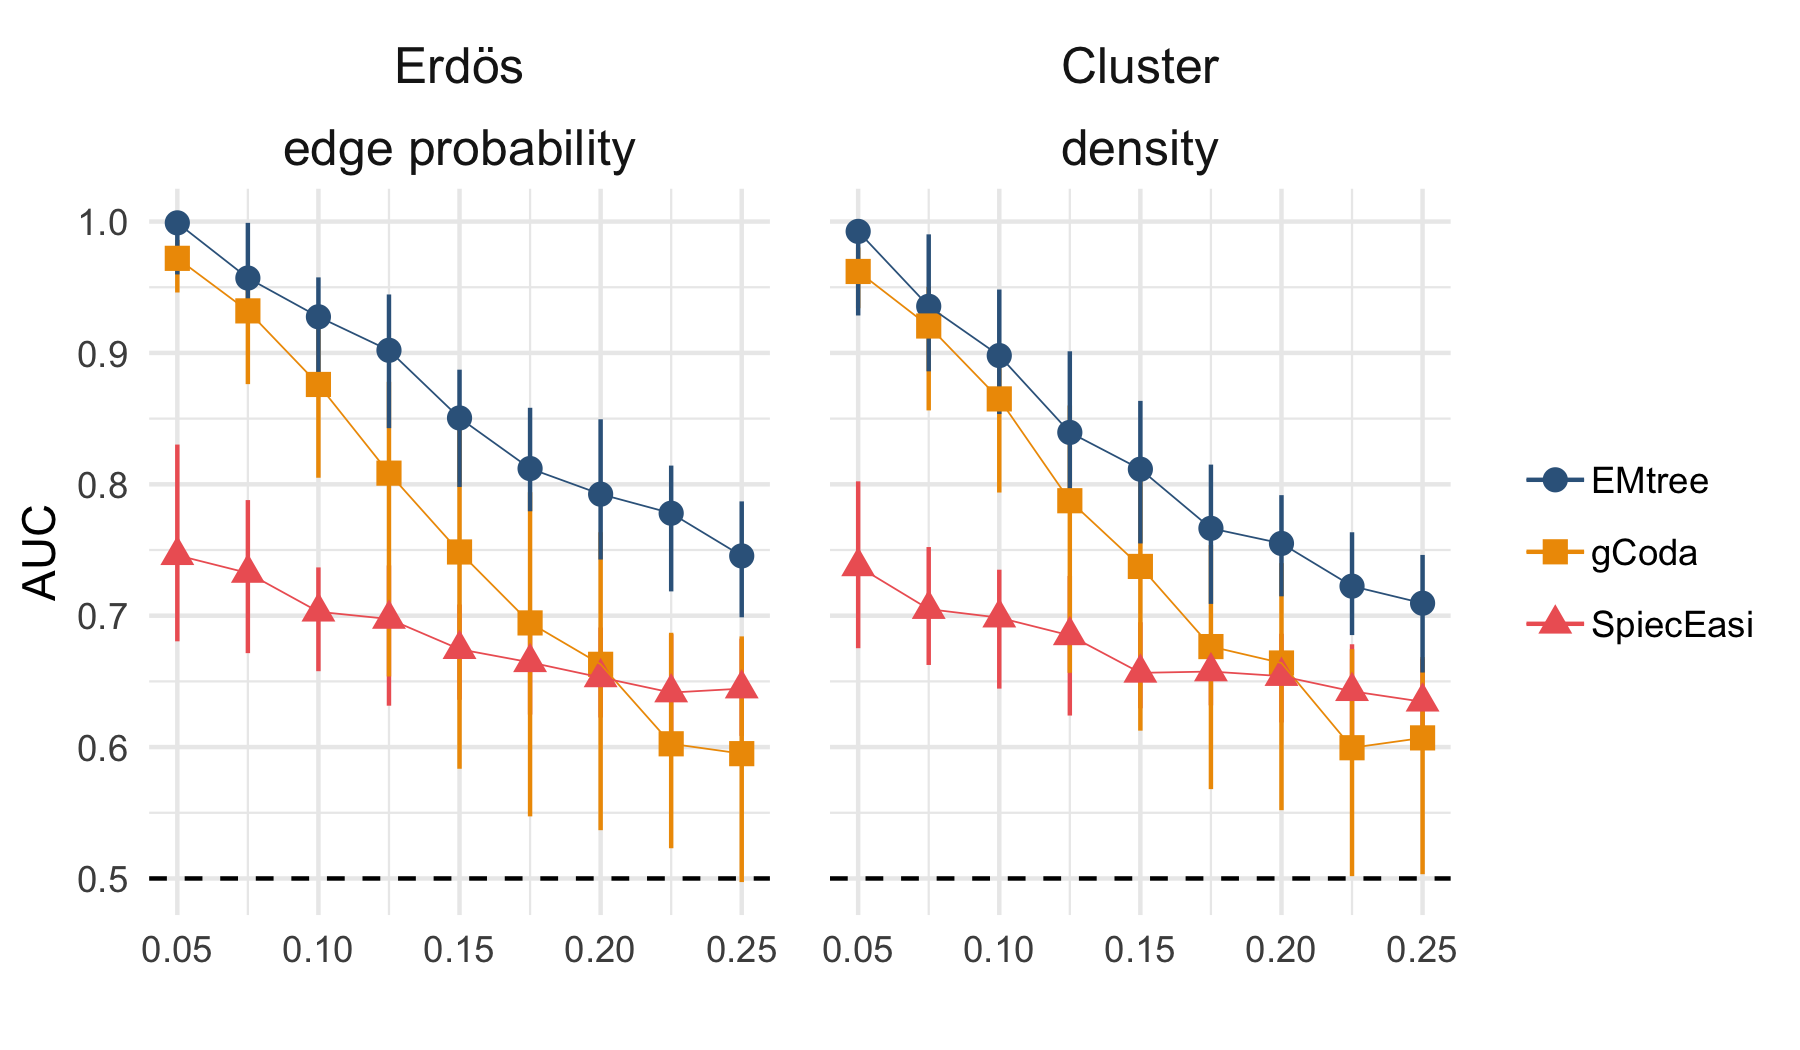
\includegraphics[width=8cm]{panel_dens.png}
  \caption{\scriptsize{Effect of graph density on the evolution of AUC median and inter-quartile intervals in Erdös and Cluster structures. (100 observations, 20 species)}}
\end{figure}
$\Rightarrow$ The tree assumption does not alter the performance
\end{frame}
%====================================================================
%====================================================================

\section{}\subsection{}

\begin{frame}{To be published soon}
    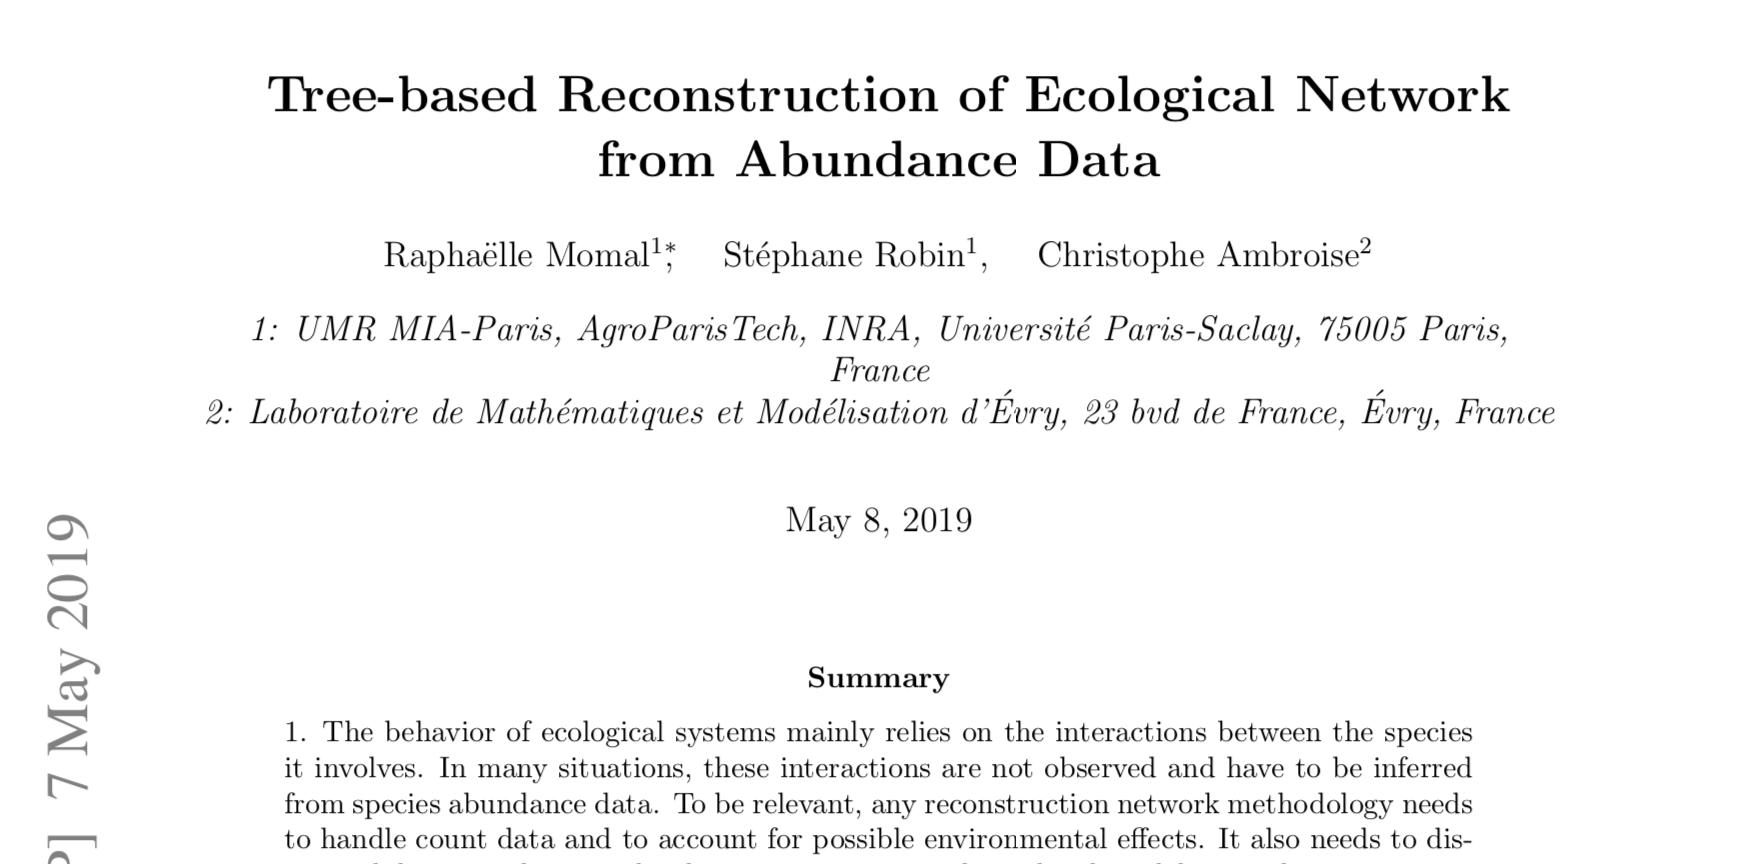
\includegraphics[width=\linewidth]{articleimag.png}
    New title: \textit{Tree-based Inference of Species Interaction Network from Abundance Data"}
\end{frame}
%-----------------------------
%---------------------------
\section{}
\begin{frame}{Conclusion}
\begin{description}
\item[Contributions:] 
\begin{itemize}
\item[]  
	\item Formal probabilistic model for network inference from count data
	\item R package: \footnotesize{\url{https://github.com/Rmomal/EMtree}}
	\item \normalsize{Preprint:} \footnotesize{\textit{Tree-based Reconstruction of Ecological Network from Abundance Data.}} \footnotesize{\url{https://arxiv.org/pdf/1905.02452.pdf}}
	
	
\end{itemize}
\bigskip 
\item[Perspectives:]

\begin{itemize}
\item[]  
	\item Sign and strength of interactions according to graphical models theory
	\item Missing major actor (species/covariates)	
	\item More collaborations with experts in macro-ecology field
\end{itemize}
\end{description}
\end{frame}
%====================================================================
%====================================================================


\begin{frame}{}

\begin{center}
\huge{Thank you}    
\end{center}

\bigskip
\bigskip

\small{
Contact :\\
\begin{description}
\item[email] raphaelle.momal@agroparistech.fr
\item[Web]Rmomal.github.io
\item[Twitter] @MomalRaphaelle\\
\end{description}}
\begin{center}
	
\includegraphics[width=0.25\linewidth]{logo_inra.jpg}\hspace{0.1cm}
	
\includegraphics[width=0.25\linewidth]{agro.PNG}
	
\includegraphics[width=0.25\linewidth]{lmh.png}\hspace{0.1cm}
	
\includegraphics[width=0.15\linewidth]{upsud.jpg}
    
\end{center}

\end{frame}

%====================================================================
%====================================================================
%====================================================================
%====================================================================
%====================================================================
%====================================================================

\appendix
\backupbegin
\begin{frame}[allowframebreaks]
\bibliographystyle{apalike}
{\tiny
    \bibliography{biblio3.bib}}
\frametitle{References}
%\bibliography{cellcite}
\end{frame}\backupend




\section{ }
\subsection{ }
\begin{frame}{Conditional probability computation}
\footnotesize
\begin{exampleblock}{Kirchhoff's theorem (matrix tree, \cite{AiH89})}
For all $W=(a_{kl})_{k,l}$ a symmetric matrix, the corresponding Laplacian $Q(W)$ is defined as follows:
 \[\mathcal{Q}_{uv}(W)=
 \begin{cases}
     -a_{uv} & 1\leq u<v \leq n\\
    \sum_{i=1}^n a_{vi} & 1\leq u=v \leq n.
\end{cases}
\]
Then for all $u$ et $v$:
    \[ |Q^*_{uv}(W)|=\sum_{T\in\mathcal{T}} \prod_{\{k,l\}\in E_T} a_{kl} \]
\end{exampleblock}
\begin{align*}
  \mathds{P}((k,l)\in T | Z)&=\sum_{T\in \mathcal{T} : (k,l)\in T}\mathds{P}( T | Z) = \frac{\sum_{(k,l)\in T} \mathds{P}(T)\mathds{P}(Z|T)}{\sum_{T} \mathds{P}(T)\mathds{P}(Z|T)}\\
 &=\emphase{1- \frac{|Q^*_{uv}(\beta\Psi^{-kl})|}{|Q^*_{uv}(\beta\Psi)|}}\\
 &= \tau_{kl}
 \end{align*}
 
\end{frame}



%====================================================================
%====================================================================

%====================================================================
%====================================================================

\begin{frame}{Direct EM algorithm ?}
\footnotesize 
\begin{itemize}
    \item \bleu{Complete likelihood :}

 \[ \mathds{P}(Y,Z,T) = \color{olive}\mathds{P}(T)\color{black}\times\color{blue}\mathds{P}(Z|T)\color{black}\times\color{orange}\mathds{P}(Y|Z)\]
 
\begin{align*}
 \log(\mathds{P}(Y,Z,T)) &= \sum_{k,l} \mathds{1}_{\{(k,l) \in T\}} (\color{olive}\log(\beta_{kl})\color{black} + \color{blue}\log(\psi_{kl}(Z)) \color{black})-\color{olive}\log(B)\color{black} \\
 &+\sum_k (\color{blue} \log(\mathds{P}(Z_k))\color{black} + \color{orange}\log(\mathds{P}(Y_k|Z_k))\color{black})
 \end{align*}
 
 \pause
 \item \bleu{Conditional expectation :}
\end{itemize}
\begin{align*}
    \mathds{E}_\theta[\log(\mathds{P}(Y,Z,T))|Y] =&\sum_{k,l\in V} \mathds{P}((k,l) \in T|Y) \log(\beta_{kl}) + \mathds{E}[\mathds{1}_{\{(k,l) \in T\}}\emphase{\log(\psi_{kl}(Z)|Y)}]\\
& +\sum_k \emphase{\mathds{E}[\log(\mathds{P}(Z_k)) | Y]} + \mathds{E}[\log(\mathds{P}(Y_k|Z_k)) | Y]-\log(B)
\end{align*} 

\normalsize 
\end{frame}
%====================================================================
%====================================================================
\begin{frame}{Maximum likelihood with hidden data}
  $$    \left.
   \begin{array}{cc}
    \text{observations } Y \\
    \text{hidden parameters } H 
   \end{array}
   \right\}\Rightarrow \log p(Y) \text{ intractable.}$$\\
   
   \bigskip   \bigskip
   
   \bleu{EM algorithm} maximizes a surrogate for the log-likelihood :
   $$Q = \mathds{E} [\log p (Y,H)|Y] = \int \log p(Y,h)p(h|Y) dh $$
   
   In most cases the conditional density $p(h|Y)$ is intractable.
    
    \bigskip    \bigskip
    
   \bleu{Variational EM} (VEM) resorts to a proxy $q(h)=\tilde{p}(h|Y)$.
\end{frame}

%====================================================================
%====================================================================

\end{document}